% !TeX root = index.tex
\documentclass[a4paper, 12pt]{report}		% general format

%%%% Charset
\usepackage{cmap}							% make PDF files searchable and copyable
\usepackage[utf8]{inputenc}					% accept different input encodings
\usepackage[T2A]{fontenc}					% russian font
\usepackage[russian]{babel}					% multilingual support (T2A)

%%%% Graphics
\usepackage[dvipsnames]{xcolor}			% driver-independent color extensions
\usepackage{graphicx}						% enhanced support for graphics
\usepackage{wrapfig}						% pro­duces fig­ures which text can flow around

%%%% Math
\usepackage{amsmath}						% Amer­i­can Math­e­mat­i­cal So­ci­ety (AMS) math fa­cil­i­ties
\usepackage{amsfonts}						% fonts from the AMS
\usepackage{amssymb}						% additional math symbols

%%%% Ty­po­grapy (don't forget about cm-super)
\usepackage{microtype}						% sublim­i­nal re­fine­ments to­wards ty­po­graph­i­cal per­fec­tion
\linespread{1.3}							% line spacing
\usepackage[left=2.5cm, right=1.5cm, top=2.5cm, bottom=2.5cm]{geometry}
\setlength{\parindent}{0pt}					% we don't want any paragraph indentation
\setlength{\parskip}{0.3cm}
\renewcommand{\chaptername}{}

%%%% Other
\usepackage{hyperref}							% ver­ba­tim with URL-sen­si­tive line breaks
\usepackage{fancyvrb}
%\DeclareUnicodeCharacter{00A0}{~}
\usepackage{float}

%------------------------------------------------------------------------------
\usepackage{listings}						% type­set source code list­ings

% Цвета для кода
\definecolor{string}{HTML}{101AF9}			% цвет строк в коде
\definecolor{comment}{HTML}{3F7F5F}		% цвет комментариев в коде
\definecolor{keyword}{HTML}{5F1441}		% цвет ключевых слов в коде
\definecolor{morecomment}{HTML}{8000FF}	% цвет include и других элементов в коде
\definecolor{captiontext}{HTML}{FFFFFF}	% цвет текста заголовка в коде
\definecolor{captionbk}{HTML}{999999}		% цвет фона заголовка в коде
\definecolor{bk}{HTML}{FFFFFF}				% цвет фона в коде
\definecolor{frame}{HTML}{999999}			% цвет рамки в коде

% Настройки отображения кода
\lstset{
	language=C++,							% Язык кода по умолчанию
	morekeywords={*,...},					% если хотите добавить ключевые слова, то добавляйте
	% Цвета
	keywordstyle=\color{keyword}\ttfamily\bfseries,
	stringstyle=\color{string}\ttfamily,
	commentstyle=\color{comment}\ttfamily\itshape,
	morecomment=[l][\color{morecomment}]{\#},
	% Настройки отображения
	breaklines=true,						% Перенос длинных строк
	basicstyle=\ttfamily\footnotesize,		% Шрифт для отображения кода
	backgroundcolor=\color{bk},				% Цвет фона кода
	%frame=lrb,xleftmargin=\fboxsep,xrightmargin=-\fboxsep, % Рамка, подогнанная к заголовку
	frame=tblr								% draw a frame at all sides of the code block
	rulecolor=\color{frame},				% Цвет рамки
	tabsize=2,								% tab space width
	showstringspaces=false,					% don't mark spaces in strings
	% Настройка отображения номеров строк. Если не нужно, то удалите весь блок
	numbers=left,							% Слева отображаются номера строк
	stepnumber=1,							% Каждую строку нумеровать
	numbersep=5pt,							% Отступ от кода
	numberstyle=\small\color{black},		% Стиль написания номеров строк
	% Для отображения русского языка
	extendedchars=true,
    literate=
        {Ö}{{\"O}}1                    {Ä}{{\"A}}1                    {Ü}{{\"U}}1
        {ß}{{\ss}}1                    {ü}{{\"u}}1                    {ä}{{\"a}}1
        {ö}{{\"o}}1                    {~}{{\textasciitilde}}1        {а}{{\selectfont\char224}}1
        {б}{{\selectfont\char225}}1    {в}{{\selectfont\char226}}1    {г}{{\selectfont\char227}}1
        {д}{{\selectfont\char228}}1    {е}{{\selectfont\char229}}1    {ё}{{\"e}}1
        {ж}{{\selectfont\char230}}1    {з}{{\selectfont\char231}}1    {и}{{\selectfont\char232}}1
        {й}{{\selectfont\char233}}1    {к}{{\selectfont\char234}}1    {л}{{\selectfont\char235}}1
        {м}{{\selectfont\char236}}1    {н}{{\selectfont\char237}}1    {о}{{\selectfont\char238}}1
        {п}{{\selectfont\char239}}1    {р}{{\selectfont\char240}}1    {с}{{\selectfont\char241}}1
        {т}{{\selectfont\char242}}1    {у}{{\selectfont\char243}}1    {ф}{{\selectfont\char244}}1
        {х}{{\selectfont\char245}}1    {ц}{{\selectfont\char246}}1    {ч}{{\selectfont\char247}}1
        {ш}{{\selectfont\char248}}1    {щ}{{\selectfont\char249}}1    {ъ}{{\selectfont\char250}}1
        {ы}{{\selectfont\char251}}1    {ь}{{\selectfont\char252}}1    {э}{{\selectfont\char253}}1
        {ю}{{\selectfont\char254}}1    {я}{{\selectfont\char255}}1    {А}{{\selectfont\char192}}1
        {Б}{{\selectfont\char193}}1    {В}{{\selectfont\char194}}1    {Г}{{\selectfont\char195}}1
        {Д}{{\selectfont\char196}}1    {Е}{{\selectfont\char197}}1    {Ё}{{\"E}}1
        {Ж}{{\selectfont\char198}}1    {З}{{\selectfont\char199}}1    {И}{{\selectfont\char200}}1
        {Й}{{\selectfont\char201}}1    {К}{{\selectfont\char202}}1    {Л}{{\selectfont\char203}}1
        {М}{{\selectfont\char204}}1    {Н}{{\selectfont\char205}}1    {О}{{\selectfont\char206}}1
        {П}{{\selectfont\char207}}1    {Р}{{\selectfont\char208}}1    {С}{{\selectfont\char209}}1
        {Т}{{\selectfont\char210}}1    {У}{{\selectfont\char211}}1    {Ф}{{\selectfont\char212}}1
        {Х}{{\selectfont\char213}}1    {Ц}{{\selectfont\char214}}1    {Ч}{{\selectfont\char215}}1
        {Ш}{{\selectfont\char216}}1    {Щ}{{\selectfont\char217}}1    {Ъ}{{\selectfont\char218}}1
        {Ы}{{\selectfont\char219}}1    {Ь}{{\selectfont\char220}}1    {Э}{{\selectfont\char221}}1
        {Ю}{{\selectfont\char222}}1    {Я}{{\selectfont\char223}}1    {і}{{\selectfont\char105}}1
        {ї}{{\selectfont\char168}}1    {є}{{\selectfont\char185}}1    {ґ}{{\selectfont\char160}}1
        {І}{{\selectfont\char73}}1     {Ї}{{\selectfont\char136}}1    {Є}{{\selectfont\char153}}1
        {Ґ}{{\selectfont\char128}}1
}

% Для настройки заголовка кода
\usepackage{caption}
\DeclareCaptionFont{white}{\color{сaptiontext}}
\DeclareCaptionFormat{listing}{\parbox{\linewidth}{\colorbox{сaptionbk}{\parbox{\linewidth}{#1#2#3}}\vskip-4pt}}
%\captionsetup[lstlisting]{format=listing,labelfont=white,textfont=white}
\renewcommand{\lstlistingname}{Листинг} % Переименование Listings в нужное именование структуры

%------------------------------------------------------------------------------
\begin{document}

\begin{titlepage}

%----------------------------------------------------------------------------------------
%	HEADING SECTIONS
%----------------------------------------------------------------------------------------
\begin{center} % Center everything
Федеральное государственное автономное образовательное \\
учреждение высшего образования \\[0.4cm]
% https://www.spbstu.ru/university/organizational-documents/corporate-identity/

\includegraphics[scale=0.8]{res/SPbPU-logo} \\[0.4cm]
Институт компьютерных наук и технологий \\*
Высшая школа интеллектуальных систем и суперкомпьютерных технологий
\end{center}

\vspace{3cm}

%----------------------------------------------------------------------------------------
%	TITLE SECTION
%----------------------------------------------------------------------------------------
\begin{center} % Center everything
\textbf{Курсовая работа}\\
по дисциплине "Сетевая безопасность"\\
на тему\\
\textbf{Исследование коммуникационного протокола WebSocket}
\end{center}

\vspace{3.5cm}
 
%----------------------------------------------------------------------------------------
%	AUTHOR SECTION
%----------------------------------------------------------------------------------------
\begin{flushleft}
Выполнил студент гр. 3540901/21501 \hspace{3cm} $\underset{\text{(подпись)}}{\underline{\hspace{3cm}}}$ С.А.Мартынов\\[0.5cm]
Преподаватель \hspace{7.25cm} $\underset{\text{(подпись)}}{\underline{\hspace{3cm}}}$ В.Э. Шмаков\\[0.5cm]
\hspace{10.2cm} «\underline{\hspace{1cm}}» \underline{\hspace{3cm}} 2023 г.
\end{flushleft}

\vfill % Fill the rest of the page with whitespace

%----------------------------------------------------------------------------------------
%	DATE SECTION
%----------------------------------------------------------------------------------------
\begin{center}
Санкт-Петербург\\
2023
\end{center}

\end{titlepage}

\setcounter{page}{2}                            % inclide the title page
\tableofcontents
\chapter*{Лабораторная работа 1. Сокетные соединения}
\addcontentsline{toc}{chapter}{Лабораторная работа 1. Сокетные соединения}

\textbf{Цель работы:} Освоение набора системных вызовов для создания сокетных соединений различных типов, для обмена данными на хостах и по сети.

\section*{1. Системные вызовы}
\textbf{Задача:} Проанализируйте набор системных вызовов для серверной и клиентской сторон при организации соединений на сокетах под ОС Linux, принимая во внимание возможности различных видов сокетов и семейств адресации.

\textbf{Ход решения:}

Основные вызовы:
\begin{itemize}
    \item \texttt{socket()} -- создать новый сокет и вернуть файловый дескриптор;
    \item \texttt{send()} -- отправить данные по сети;
    \item \texttt{receive()} -- получить данные из сети;
    \item \texttt{close()} -- закрыть соединение.
\end{itemize}

Основные вызовы на стороне сервера:
\begin{itemize}
    \item \texttt{bind()} -- связать сокет с IP-адресом и портом;
    \item \texttt{listen()} -- слушает порт и ждет когда будет установлено соединение;
    \item \texttt{accept()} -- принять запрос на установку соединения.
\end{itemize}

Основные вызовы на стороне клиента:
\begin{itemize}
    \item \texttt{connect()} -- установить соединение.
\end{itemize}

Основные семейства протоколов создаваемого сокета:
\begin{itemize}
    \item \texttt{AF\_INET} -- для сетевого протокола IPv4;
    \item \texttt{AF\_INET6} -- для IPv6;
    \item \texttt{AF\_UNIX} -- для локальных сокетов (используя файл).
\end{itemize}

Основные типы соединений:
\begin{itemize}
    \item \texttt{SOCK\_STREAM} -- надёжная потокоориентированная служба или потоковый сокет;
    \item \texttt{SOCK\_DGRAM} -- служба датаграмм или датаграммный сокет;
    \item \texttt{SOCK\_RAW} -- сырой протокол поверх сетевого уровня.
\end{itemize}

\section*{2. Присоединенные сокеты}
\textbf{Задача:} Скомпилируйте и выполните программу \texttt{socketpair.cpp}, иллюстрирующую создание простейшего вида сокета и обмен данными двух родственных процессов.

Проанализируйте вывод на консоль. Существует ли зависимость обмена от различных соотношений величин временных задержек (в вызовах \texttt{sleep()}) в процессе-родителе и в процессе-потомке?

\textbf{Ход решения:} Беглый анализ исходного текста позволяет выявить следующие моменты:
\begin{enumerate}
    \item{В цикле \texttt{switch} дан не правильный комментарий для поведения по умолчанию: там сказано, что дальнейший код будет исполняться потомком, хотя это не так. Системный вызов \texttt{fork()} возвращает положительное не нулевое число для процесса-родителя.}
    \item{Для организации сетевого взаимодействия используется системный вызов \texttt{socketpair()}, который создает пару безымянных присоединённых сокетов. Рассмотрим параметры, которые используются для этого системного вызова:
                \begin{itemize}
                    \item \texttt{PF\_UNIX} показывает, что будет использовано локальное соединение.
                    \item \texttt{SOCK\_STREAM} показывает, что семантика коммуникации обеспечивает создание двусторонних надежных и последовательных потоков байтов, поддерживающих соединения.
                \end{itemize}
                Остальные параметры тривиальны.
          }
    \item{Учитывая, что потомок всегда пишет, и только потом читает, а предок действует наоборот, и при этом у нас блокирующие операции, сразу понятно, что будет простой поочерёдный обмен, и вызов \texttt{sleep()} ни на что не влияет. Или, другими словами, каждый этот вызов будет влиять и на одну и на другую сторону общения, увеличивая их ожидание.}
\end{enumerate}

\textbf{Эксперимент:} Запустив приложение, мы получили следующий вывод:
\begin{Verbatim}[frame=single]
    smart@thinkpad$ ./socketpair
    p->c:0
    c->p: 1
    p->c:2
    c->p: 3
    p->c:4
    c->p: 5
    p->c:6
    c->p: 7
    p->c:8
    c->p: 9
\end{Verbatim}

Дальнейшие эксперименты с \texttt{sleep()} подтвердили изначальные гипотезы: можно полностью убрать оба вызова \texttt{sleep()} и это не сломает программу, можно увеличивать значение параметра для \texttt{sleep()} и это будет влиять на оба процесса.

\section*{3. Локальные сокеты}
\textbf{Задача:} Скомпилируйте программы \texttt{echo\_server.cpp} и \texttt{echo\_client.cpp}, задавая им при компиляции разные имена.

Запустите программы сервера и клиента на разных терминалах. Введите символьную информацию в окне клиента и проанализируйте вывод. Какой разновидности принадлежат сокеты, используемые в данном примере клиент-серверного взаимодействия?

С чем связано создание специального файла в текущем каталоге во время исполнения программ?

\textbf{Ход решения:} Начнём с анализа исходных кодов.

Сервер:
\begin{enumerate}
\item Создаётся сокет, используя системный вызов \texttt{socket()}. Параметры \texttt{AF\_UNIX} и \texttt{SOCK\_STREAM} идентичны параметрам из предыдущего шага (\texttt{AF\_UNIX} это синоним для \texttt{PF\_UNIX}). Фактический результат этого вызова -- файловый дескриптор.
\item Для соединения (\texttt{bind()}) сокета с адресом (\texttt{sockaddr\_un}), производится подготовка этого адреса. Обычно тут задаётся адрес хоста и номер порта для ожидания соединения, но в данном случае адресу задаётся семейство, идентичное семейству сокета (\texttt{AF\_UNIX}) и указывается путь, где сокет будет располагаться в файловой системе. Вызов (\texttt{unlink()}) позволяет автоматически удалить файл сокета, когда он перестанет использоваться.
\item После связывания, сокет переводится в режим прослушивания (\texttt{listen()}). Число 5 позволяет размер очереди клиентов, желающих подключиться.
\item В бесконечном цикле, сервер ожидает подключения клиента. Исполнение процесса будет заблокировано на вызове \texttt{accept()}. Этот вызов позволяет позволяет получить копию исходного сокета, чтобы слушающий сокет был готов к получению запросов от других клиентов.
\item После этого снова в бесконечном цикле происходит получение и отправка сообщений длинной в 100 символов через копию сокета, полученного на предыдущем шаге.
\end{enumerate}

клиент:
\begin{enumerate}
\item Подобно серверу, создаётся сокет, используя системный вызов \texttt{socket()} с параметрами \texttt{AF\_UNIX} и \texttt{SOCK\_STREAM}.
\item На клиенте идёт подготовка к соединению. Обычно используется имя удалённого хоста и номер порта. Однако в нашем случае используется адрес сокета в файловой системе (адрес записывается в структуру \texttt{sockaddr\_un}).
\item Дальше следует непосредственно соединение (\texttt{connect()}).
\item В бесконечном цикле происходит считывание данных с устройства ввода (\texttt{stdin}), отправка их серверу, получение ответа от сервера и вывод этого ответа на стандартное устройство вывода (\texttt{stdout}).
\end{enumerate}

\textbf{Эксперимент:} Запуск сервера:
\begin{Verbatim}[frame=single]
    smart@thinkpad$ ./echo_server
    Waiting for a connection...
\end{Verbatim}

Запуск клиента:
\begin{Verbatim}[frame=single]
    smart@thinkpad$ ./echo_client
    Trying to connect...
    Connected.
    > 123
    echo> 123
    > test
    echo> test
    > тест
    echo> тест
    > ~!@#$%
    echo> ~!@#$%
    > 
\end{Verbatim}

После запуска сервера, в директории появляется файл сокета. Инормацию о нём можно получить, к примеру, с помощью утилиты \texttt{ss}.
\begin{Verbatim}[frame=single]
smart@thinkpad$ ss | grep echo_socket
u_str ESTAB    0      0               echo_socket 481033            * 481088
\end{Verbatim}
Эта запись означает следующее:
\begin{itemize}
    \item \texttt{u\_str} -- сетевой идентификатор;
    \item \texttt{ESTAB} -- состояние соединения;
    \item 0 -- количество пакетов в очереди на получение (\texttt{Recv-Q});
    \item 0 -- количество пакетов в очереди на отправку (\texttt{Send-Q});
    \item echo\_socket 481033 -- локальный адрес и порт (большое число для локальных соединений);
    \item $\ast{}$ 481088 -- адрес и порт клиента.
\end{itemize}

\section*{4. Интернет сокеты}
\textbf{Задача:} Скомпилируйте c разными именами программы \texttt{sock\_c\_i\_srv.cpp} и \texttt{sock\_c\_i\_clt.cpp} (в них используется общий \texttt{include} файл \texttt{local\_c\_i.h}). Запустите программы сервера и клиента на разных терминалах. При запуске клиента указывайте в качестве параметра командной строки имя хоста \texttt{localhost}. Введите символьную информацию в окне клиента и поясните вывод.

Какой разновидности принадлежат сокеты, используемые в данном примере клиент-серверного взаимодействия?

\textbf{Ход решения:} Проведём анализ кода. Алгоритм практически аналогичен предыдущему примеру, но тут используется семейство \texttt{AF\_INET} и создание отдельных процессов для обслуживания клиентов. В данном примере, мы как и раньше используем потоковую передачу (\texttt{SOCK\_STREAM}), однако сетевые сокеты позволяют организовать передачу на датаграммах (\texttt{SOCK\_STREAM}) -- такие соединения работают без подтверждения факта доставки (\texttt{ACK}).

И сервер и клиент при вызове функции \texttt{socket()} используют константу \texttt{AF\_INET}, указывающую на то, что открываемый сокет должен быть сетевым. Сокеты в домене \texttt{AF\_INET}, не знают про то, что они работают на локальной системе и обращаются только к \texttt{localhost}. Они полностью выполняют все механизмы сетевого стека: переключения контекста, \texttt{ACK}, \texttt{TCP}, управление потоком, маршрутизацию, разбиение больших пакетов и т.п. То есть это «полноценная TCP работа» несмотря на то, что пакеты не покидают локального интерфейса.

Дополнительные издержки при использовании \texttt{AF\_INET} кроются так же в необходимости произвести резолвинг доменного имени в IP-адрес (вызов \texttt{gethostbyname()}) и решение проблемы little-big-end (вызов \texttt{htons()}, \texttt{htonl()}) связанной с разным порядком байтов на различных архитектурах (в комментариях кода написано что-то странное про "fake port").

Ещё одной особенность является обработка подключений клиентов в отдельных процессах. После установки соединения, сервер вызывает \texttt{fork()} и работает с каждым клиентом отдельно. Это значит, что каждый клиент получит в ответ только свои сообщения.

\textbf{Эксперимент:} запуск сервера.
\begin{Verbatim}[frame=single]
    smart@thinkpad$ ./sock_c_i_srv 
\end{Verbatim}

Запуск первого клиента.
\begin{Verbatim}[frame=single]
    smart@thinkpad$ ./sock_c_i_clt localhost
    > 1
    1
    > 2
    2
    > 3
    3
    > 
\end{Verbatim}

Запуск второго клиента.
\begin{Verbatim}[frame=single]
    smart@thinkpad$ ./sock_c_i_clt localhost
    > a
    A
    > b
    B
    > c
    C
    > d
    D
    > 
\end{Verbatim}

Замена строчных букв на заглавные происходит на стороне сервера при помощи команды \texttt{toupper(buf[i])}.

\section*{5. Модификация эхо-сервера}
\textbf{Задача:} Модифицируйте программу \texttt{echo\_server.cpp} так, чтобы при ответе на запросы клиента что-либо выводилось в окне сервера.

Испытайте работу эхо-сервера при работе с несколькими клиентами.

\textbf{Ход решения:}

Фактически, была добавлена только строчка 3, представленная в листинге 1.

\lstinputlisting[language=C++, caption={Фрагмент исходного кода модифицированного файла (echo\_server\_upd.cpp)}, firstline=69, lastline=79]
{../Tasks/1_Network_application/source_files/echo_server_upd.cpp}

\textbf{Эксперимент:} запуск сервера.
\begin{Verbatim}[frame=single]
    smart@thinkpad$ ./echo_server_upd 
    Waiting for a connection...
    Connected.
    [client 4] 1
    [client 4] 2
    [client 4] 3
    [client 4] 4
    Waiting for a connection...
    Connected.
    [client 4] a
    [client 4] b
    [client 4] c
    [client 4] d
\end{Verbatim}

Запуск первого клиента.
\begin{Verbatim}[frame=single]
    smart@thinkpad$ ./echo_client 
    Trying to connect...
    Connected.
    > 1
    echo> 1
    > 2
    echo> 2
    > 3
    echo> 3
    > 4
    echo> 4
    > ^C
\end{Verbatim}

Запуск второго клиента.
\begin{Verbatim}[frame=single]
    smart@thinkpad$ ./echo_client 
    Trying to connect...
    Connected.
    > a
    b
    c
    d
    echo> a
    > echo> b
    > echo> c
    > echo> d
    > 
\end{Verbatim}

Наблюдаемое поведение полностью в рамках ожиданий: когда сервер установил соединение с первым клиентом, он находится в заблокированном состоянии на операции сетевого обмена. Как только первый клиент завершает свою работу, мгновенно происходит подключение и обслуживание второго клиента (он даже получает тот-же номер файлового дескриптора). Отсюда напрашивается вывод, что работа слушающего сокета должна производиться в одном потоке, а обслуживающих -- в другом (других).
\chapter*{Лабораторная работа 2. Сокеты L4}
\addcontentsline{toc}{chapter}{Лабораторная работа 2. Сокеты L4}

\textbf{Цель работы:} Создание клиент-серверных приложений, взаимодействующих друг с другом по сети на основе технологии соединения на сокетах L4.

\section*{1. Анализ кода}
\textbf{Задача:} Проанализируйте код программы \texttt{server\_game.cpp}, иллюстрирующей обмен данными с клиентскими приложениями по итеративной схеме.

\textbf{Ход решения:} Используется сокет семейства \texttt{AF\_INET}. Сервер ожидает соединения на любом IP адресе (\texttt{INADDR\_ANY}), но нам достаточно для подключения \texttt{localhost}. Для соединения будет использоваться порт 1066. Игра работает в один поток.

\section*{2. Компиляция и запуск}
\textbf{Задача:} Скомпилируйте и запустите \texttt{server\_game}.

\textbf{Эксперимент:} запуск сервера.
\begin{Verbatim}[frame=single]
    smart@thinkpad$ g++ server_game.cpp -o server_game
    smart@thinkpad$ ./server_game 
    start to listen

\end{Verbatim}

Системный журнал зафиксировал выбор слова сервером.
\begin{Verbatim}[frame=single]
    smart@thinkpad$ journalctl -a | grep server_game
    Feb 08 23:43:25 thinkpad server_game[103180]: server_game chose word green
    Feb 08 23:43:40 thinkpad server_game[103180]: server_game chose word green
\end{Verbatim}

\section*{3. Анализ состояния сокета}
\textbf{Задача:} Запустите другой терминал и проверьте с него наличие в системе созданного сервером сокета и то, что он находится в состоянии \texttt{LISTEN}. Для этого выполните команду \texttt{netstat -a | grep 1066}.

Проанализируйте вывод данной команды и объясните ее смысл.

\textbf{Ход решения:} Так как команда \texttt{netstat} устарела и была заменена на \texttt{ss}, то будет рассматривать вывод \texttt{ss -atp | grep game}

\textbf{Эксперимент:} результат запуска команды \texttt{ss}
\begin{Verbatim}[frame=single]
    smart@thinkpad$ ss -atp | grep game
    State  Recv-Q Send-Q Local Address:Port       Peer Address:PortProcess
    LISTEN 0      5            0.0.0.0:fpo-fns         0.0.0.0:*    users:(("server_game",pid=103180,fd=3))
\end{Verbatim}

В результате мы видим, что в данный момент сокет находится в состоянии \texttt{LISTEN}. В очереди на получение находятся 0 покетов, на отправку 5. Сервер слушает на любом адресе, но вместо номера порта мы видим \texttt{fpo-fns}. Порт 1066 зарезервирован в системе для какой-то компьютерной игры, поэтому мы видем название вместо номера. Дальше мы видим, что клиент пока не подключился. А в самом конце строки общую информацию о процессе.

\section*{4. Присоединенные сокеты}
\textbf{Задача:} Запустите в качестве клиентского процесса утилиту \texttt{telnet} с параметрами: \texttt{telnet localhost 1066}. При организации коммуникации по сети на разных компьютерах вместо \texttt{localhost} при запуске клиента указывается IP-адрес компьютера, на котором был запущен сервер.

\textbf{Ход решения:} Ввиду устаревания \texttt{telnet}, воспользуемся утилитой \texttt{gnu netcat}.

\textbf{Эксперимент:} Запуск клиента
\begin{Verbatim}[frame=single]
    smart@thinkpad$ nc localhost 1066
    :laying on host: h
\end{Verbatim}
Программа запустилось, соединение установленго. Но имя хости на сервере ничем не инициализированно.

\section*{5. Игра}
\textbf{Задача:} Диалог с сервером заключается в угадывании слова. Оно вводится по буквам с клиентского терминала. При этом сервер вместо неугаданных букв выдает символы \texttt{”-”}, а также считает число оставшихся неудачных попыток (всего их предусмотрено 12).

\textbf{Эксперимент:} Запуск клиента
\begin{Verbatim}[frame=single]
    smart@thinkpad$ nc localhost 1066
    :laying on host: h
    
     -----   12
    ф
     -----   11
    g
     g----   11
    r
     gr---   11
    e
     gree-   11
    e
     gree-   11
    b
     gree-   10
    n
     green   10
    
     green   9
\end{Verbatim}

Заметно, что логика игры не доделана: победная ситуация не обрабатывается корректно.

\section*{6. Состояние сокета в разные моменты}
\textbf{Задача:} Завершите серверное приложение с помощью сигнала \texttt{kill}, и затем определите командой \texttt{netstat -a | grep 1066}, когда исчезает из системы соединение на сокетах. Во время сеанса обмена также примените команду \texttt{netstat -a | grep 1066}, чтобы исследовать состояние соединения.

\textbf{Эксперимент:} Состояние сокета после завершения игры
\begin{Verbatim}[frame=single]
    smart@thinkpad$ ss -atp | grep game
    State  Recv-Q Send-Q Local Address:Port       Peer Address:PortProcess
\end{Verbatim}
Сокет не обнаружен.

Состояние сокета в процессе игры
\begin{Verbatim}[frame=single]
    smart@thinkpad$ ss -atp | grep game
    State  Recv-Q Send-Q Local Address:Port       Peer Address:PortProcess
    LISTEN 0      5            0.0.0.0:fpo-fns         0.0.0.0:*         users:(("server_game",pid=109301,fd=3))
    ESTAB  0      0          127.0.0.1:fpo-fns       127.0.0.1:52880     users:(("server_game",pid=109301,fd=4))
\end{Verbatim}
Как и ожидалось, мы видим один слушающий сокет, и один установленный. При этом \texttt{127.0.0.1:fpo-fns} -- данные сервера, а \texttt{127.0.0.1:52880} -- данные клиента.

\section*{7. Множество подключений}
\textbf{Задача:} Проделайте все заново, но запускайте не одно клиентское приложение (в виде \texttt{telnet}), а несколько экземпляров с разных терминалов, и попытайтесь работать с них одновременно.

Проанализируйте, как сервер будет обслуживать запросы в этом случае.

\textbf{Эксперимент:} После запуска двух дополнительных клиентов, мы видим, что они находится в состоянии блокировки на операции \texttt{connect}, и не получают сообщений от сервера.

\begin{Verbatim}[frame=single]
    smart@thinkpad$ ss -atp | grep game
    State  Recv-Q Send-Q Local Address:Port       Peer Address:PortProcess
    LISTEN 2      5            0.0.0.0:fpo-fns         0.0.0.0:*         users:(("server_game",pid=109301,fd=3))
    ESTAB  0      0          127.0.0.1:fpo-fns       127.0.0.1:52880     users:(("server_game",pid=109301,fd=4))
\end{Verbatim}
Состояние сокета показывает очередь на слушающем сокете длинной в 2.

\section*{8. Исправление игры}
\textbf{Задача:} Модифицируйте программу \texttt{server\_game.cpp} так, чтобы запросы от каждого из клиентов могли обслуживаться конкурентно, путем запуска для каждого нового соединения собственного нового процесса на сервере или потока. Проанализируйте, как обслуживаются запросы в случае конкурентной схемы работы сервера.

Возможно также улучшить качество самой игровой функции \texttt{guess\_word()} сервера.

\textbf{Ход решения:}

Обработка подключений производится в отдельном процессе
\lstinputlisting[language=C++, caption={Фрагмент исходного кода модифицированного файла игры}, firstline=60, lastline=64]
{../Tasks/2_L4_Socket_sample/source_files/server_game_upd.cpp}

Исправлены условия для определения победы
\lstinputlisting[language=C++, caption={Фрагмент исходного кода модифицированного файла игры}, firstline=73, lastline=80]
{../Tasks/2_L4_Socket_sample/source_files/server_game_upd.cpp}

\textbf{Эксперимент:}

Состояние сокета показывает успешную работу с тремя клиентами.
\begin{Verbatim}[frame=single]
    smart@thinkpad$ ss -atp | grep game
    State  Recv-Q Send-Q Local Address:Port       Peer Address:PortProcess
    LISTEN 0      5            0.0.0.0:fpo-fns         0.0.0.0:*           users:(("server_game",pid=113319,fd=3),("server_game",pid=113317,fd=3),("server_game",pid=113310,fd=3),("server_game",pid=113306,fd=3))
    ESTAB  0      0          127.0.0.1:fpo-fns       127.0.0.1:52976       users:(("server_game",pid=113310,fd=4))                                                                                                
    ESTAB  0      0          127.0.0.1:fpo-fns       127.0.0.1:52978       users:(("server_game",pid=113317,fd=4))                                                                                                
    ESTAB  0      0          127.0.0.1:fpo-fns       127.0.0.1:56378       users:(("server_game",pid=113319,fd=4))
\end{Verbatim}

Победная ситуация успешно обрабатывается, имя хоста определяется правильно.
\begin{Verbatim}[frame=single]
    smart@thinkpad$ nc localhost 1066
    Playing on host: thinkpad:
    
     -----   12
    g
     g----   12
    r
     gr---   12
    e
     gree-   12
    n
     green   12
    You ween! Congrats!
\end{Verbatim}
\chapter*{Лабораторная работа 3. Шифрование сообщений с помощью средств GNU Privacy Guard}
\addcontentsline{toc}{chapter}{Лабораторная работа 3. Шифрование сообщений с помощью средств GNU Privacy Guard}

\textbf{Цель работы:} Знакомство с возможностями утилиты GNU Privacy Guard.

\section*{1. Установка}
\addcontentsline{toc}{section}{1. Установка}
Установка утилиты не потребовалась, т.к. она уже установлена на компьютере.
\begin{Verbatim}[frame=single]
    smart@thinkpad$ pacman -Qi gnupg
    Name            : gnupg
    Version         : 2.2.40-1
    Description     : Complete and free implementation of the OpenPGP standard
    Architecture    : x86_64
    URL             : https://www.gnupg.org/
    Licenses        : BSD  custom  custom:CC0  GPL2  GPL3  LGPL3  LGPL2.1  MIT
    Groups          : None
    Provides        : None
    Depends On      : bzip2  libbz2.so=1.0-64  glibc  gnutls  libgcrypt
                      libgpg-error  libksba  libassuan  libassuan.so=0-64  npth
                      libnpth.so=0-64  pinentry  readline  libreadline.so=8-64
                      sqlite  zlib
    Optional Deps   : libldap: gpg2keys_ldap [installed]
                      libusb-compat: scdaemon
                      pcsclite: scdaemon [installed]
    Required By     : gpgme  pacman  visual-studio-code-bin
    Optional For    : None
    Conflicts With  : None
    Replaces        : None
    Installed Size  : 8.55 MiB
    Packager        : David Runge <dvzrv@archlinux.org>
    Build Date      : Fri 14 Oct 2022 02:01:35 PM MSK
    Install Date    : Mon 19 Dec 2022 11:46:09 PM MSK
    Install Reason  : Installed as a dependency for another package
    Install Script  : Yes
    Validated By    : Signature
\end{Verbatim}

Информация о текущей версии \texttt{GnuPG} и поддерживаемых криптоалгоритмах
\begin{Verbatim}[frame=single]
    smart@thinkpad$ gpg2 --version
    gpg (GnuPG) 2.2.40
    libgcrypt 1.10.1-unknown
    Copyright (C) 2022 g10 Code GmbH
    License GNU GPL-3.0-or-later <https://gnu.org/licenses/gpl.html>
    This is free software: you are free to change and redistribute it.
    There is NO WARRANTY, to the extent permitted by law.

    Home: /home/smart/.gnupg
    Supported algorithms:
    Pubkey: RSA, ELG, DSA, ECDH, ECDSA, EDDSA
    Cipher: IDEA, 3DES, CAST5, BLOWFISH, AES, AES192, AES256, TWOFISH,
            CAMELLIA128, CAMELLIA192, CAMELLIA256
    Hash: SHA1, RIPEMD160, SHA256, SHA384, SHA512, SHA224
    Compression: Uncompressed, ZIP, ZLIB, BZIP2
\end{Verbatim}

\section*{2. Генерация ключей}
\addcontentsline{toc}{section}{2. Генерация ключей}
Произведём генерацию ключей.

Для диалога генерации ключа я использую флаг \texttt{--full-generate-key}, т.к. стандартный \texttt{--gen-key} скрывает некоторые вопросы диалога используя значения по умолчанию (в частности, используется ключ длинной 3072).
\begin{Verbatim}[frame=single]
    smart@thinkpad$ gpg2 --full-generate-key
    gpg (GnuPG) 2.2.40; Copyright (C) 2022 g10 Code GmbH
    This is free software: you are free to change and redistribute it.
    There is NO WARRANTY, to the extent permitted by law.
    
    Please select what kind of key you want:
       (1) RSA and RSA (default)
       (2) DSA and Elgamal
       (3) DSA (sign only)
       (4) RSA (sign only)
      (14) Existing key from card
    Your selection? 1
    RSA keys may be between 1024 and 4096 bits long.
    What keysize do you want? (3072) 4096
    Requested keysize is 4096 bits
    Please specify how long the key should be valid.
             0 = key does not expire
          <n>  = key expires in n days
          <n>w = key expires in n weeks
          <n>m = key expires in n months
          <n>y = key expires in n years
    Key is valid for? (0) 3w
    Key expires at Sat 04 Mar 2023 05:10:43 PM MSK
    Is this correct? (y/N) y
    
    GnuPG needs to construct a user ID to identify your key.
    
    Real name: Semen Martynov
    Email address: martynov.sa@edu.spbstu.ru
    Comment: Test digital sirnature
    You selected this USER-ID:
        "Semen Martynov (Test digital sirnature) <martynov.sa@edu.spbstu.ru>"
    
    Change (N)ame, (C)omment, (E)mail or (O)kay/(Q)uit? O
    We need to generate a lot of random bytes. It is a good idea to perform
    some other action (type on the keyboard, move the mouse, utilize the
    disks) during the prime generation; this gives the random number
    generator a better chance to gain enough entropy.
    We need to generate a lot of random bytes. It is a good idea to perform
    some other action (type on the keyboard, move the mouse, utilize the
    disks) during the prime generation; this gives the random number
    generator a better chance to gain enough entropy.
    gpg: /home/smart/.gnupg/trustdb.gpg: trustdb created
    gpg: directory '/home/smart/.gnupg/openpgp-revocs.d' created
    gpg: revocation certificate stored as '/home/smart/.gnupg/openpgp-revocs.d/9DAF94FCD9CA38BFD298BD0CA0B01E0BAB2AF7C6.rev'
    public and secret key created and signed.
    
    pub   rsa4096 2023-02-11 [SC] [expires: 2023-03-04]
          9DAF94FCD9CA38BFD298BD0CA0B01E0BAB2AF7C6
    uid                      Semen Martynov (Test digital sirnature) <martynov.sa@edu.spbstu.ru>
    sub   rsa4096 2023-02-11 [E] [expires: 2023-03-04]
\end{Verbatim}

В режиме диалога, были выбраны следующие опции
\begin{itemize}
    \item Использование ключа с двумя типа шифрования (RSA и RSA)
    \item Длинна ключа в 4096 бит (с 2015-го года NIST рекомендует использовать ключи длинной в 2018 бит, но уже сейчас многие компании перешли на 4096)
    \item 3 недели в качестве срока жизни ключа (как долго он будет валиден для использования)
    \item Имя и e-main предоставленный университетом.
\end{itemize}

Дальше выполнение диалога прервалось для ввода ключевой фразы, защищающей ключи от несанкционированного использования.
\begin{center}
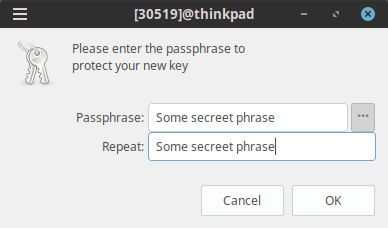
\includegraphics[scale=0.8]{res/3.pass1.png}
\end{center}

Был выбран слабый пароль для шифрования, о чём система меня предупредила. Продолжим с небезопасным паролем.
\begin{center}
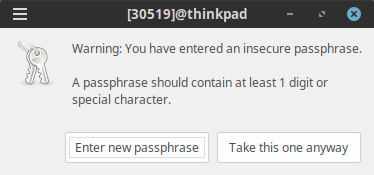
\includegraphics[scale=0.8]{res/3.pass2.png}
\end{center}

Текущий список ключей с keygrip (идемпотентный протокол хеширования для связи ключей)
\begin{Verbatim}[frame=single]
    smart@thinkpad$ gpg --list-keys --with-keygrip
    /home/smart/.gnupg/pubring.kbx
    ------------------------------
    pub   rsa4096 2023-02-11 [SC] [expires: 2023-03-04]
          9DAF94FCD9CA38BFD298BD0CA0B01E0BAB2AF7C6
          Keygrip = EC3AFAA6FD0AE71FB449D7D42849E173CF6CAAF4
    uid           [ultimate] Semen Martynov (Test digital sirnature) <martynov.sa@edu.spbstu.ru>
    sub   rsa4096 2023-02-11 [E] [expires: 2023-03-04]
          Keygrip = 16E5EFCBA47102BBA3A7C17D467D430C13D3D43E
\end{Verbatim}

\begin{itemize}
    \item \texttt{pub} -- публичный ключ (keygrip \texttt{EC3AFAA6FD0AE71FB449D7D42849E173CF6CAAF4});
    \item \texttt{uid} -- идентификатор (User-ID);
    \item \texttt{sub} -- публичный подключ (keygrip \texttt{16E5EFCBA47102BBA3A7C17D467D430C13D3D43E});
\end{itemize}

Список приватных ключей
\begin{Verbatim}[frame=single]
    smart@thinkpad$ gpg2 --list-secret-keys --with-keygrip
    /home/smart/.gnupg/pubring.kbx
    ------------------------------
    sec   rsa4096 2023-02-11 [SC] [expires: 2023-03-04]
        9DAF94FCD9CA38BFD298BD0CA0B01E0BAB2AF7C6
        Keygrip = EC3AFAA6FD0AE71FB449D7D42849E173CF6CAAF4
    uid           [ultimate] Semen Martynov (Test digital sirnature) <martynov.sa@edu.spbstu.ru>
    ssb   rsa4096 2023-02-11 [E] [expires: 2023-03-04]
        Keygrip = 16E5EFCBA47102BBA3A7C17D467D430C13D3D43E
\end{Verbatim}

\begin{itemize}
    \item \texttt{sec} -- секретный ключ (keygrip \texttt{EC3AFAA6FD0AE71FB449D7D42849E173CF6CAAF4});
    \item \texttt{uid} -- идентификатор (User-ID);
    \item \texttt{ssb} -- секретный подключ (keygrip \texttt{16E5EFCBA47102BBA3A7C17D467D430C13D3D43E});
\end{itemize}

Список подписей
\begin{Verbatim}[frame=single]
    smart@thinkpad$ gpg2 --list-signatures --with-keygrip
    /home/smart/.gnupg/pubring.kbx
    ------------------------------
    pub   rsa4096 2023-02-11 [SC] [expires: 2023-03-04]
        9DAF94FCD9CA38BFD298BD0CA0B01E0BAB2AF7C6
        Keygrip = EC3AFAA6FD0AE71FB449D7D42849E173CF6CAAF4
    uid           [ultimate] Semen Martynov (Test digital sirnature) <martynov.sa@edu.spbstu.ru>
    sig 3        A0B01E0BAB2AF7C6 2023-02-11  Semen Martynov (Test digital sirnature) <martynov.sa@edu.spbstu.ru>
    sub   rsa4096 2023-02-11 [E] [expires: 2023-03-04]
        Keygrip = 16E5EFCBA47102BBA3A7C17D467D430C13D3D43E
    sig          A0B01E0BAB2AF7C6 2023-02-11  Semen Martynov (Test digital sirnature) <martynov.sa@edu.spbstu.ru>
\end{Verbatim}

Отпечаток (fingerprint) подписи
\begin{Verbatim}[frame=single]
    smart@thinkpad$ gpg2 --fingerprint martynov.sa@edu.spbstu.ru
    pub   rsa4096 2023-02-11 [SC] [expires: 2023-03-04]
          9DAF 94FC D9CA 38BF D298  BD0C A0B0 1E0B AB2A F7C6
    uid           [ultimate] Semen Martynov (Test digital sirnature) <martynov.sa@edu.spbstu.ru>
    sub   rsa4096 2023-02-11 [E] [expires: 2023-03-04]
\end{Verbatim}

Исследуем содержимое директории \texttt{.gnupg}
\begin{Verbatim}[frame=single]
smart@thinkpad$ tree .gnupg/
.gnupg/
    openpgp-revocs.d
        9DAF94FCD9CA38BFD298BD0CA0B01E0BAB2AF7C6.rev
    private-keys-v1.d
        16E5EFCBA47102BBA3A7C17D467D430C13D3D43E.key
        EC3AFAA6FD0AE71FB449D7D42849E173CF6CAAF4.key
    pubring.kbx
    pubring.kbx~
    trustdb.gpg
\end{Verbatim}

В директории можно увидеть
\begin{itemize}
    \item \texttt{openpgp-revocs.d/9DAF94FCD9CA38BFD298BD0CA0B01E0BAB2AF7C6.rev} --  предварительно созданный сертификат отзыва. Имя файла соответствует отпечатку ключа. Всякий, у кого есть доступ к этому файлу, может отозвать соответствующий ключ.
    \item \texttt{private-keys-v1.d/EC3AFAA6FD0AE71FB449D7D42849E173CF6CAAF4.key} -- приватный ключ.
    \item \texttt{private-keys-v1.d/16E5EFCBA47102BBA3A7C17D467D430C13D3D43E.key} -- приватный подключ.
    \item \texttt{pubring.kbx} -- Таблица открытых ключей.
    \item \texttt{pubring.kbx~} -- Таблица открытых ключей (резервная копия).
    \item \texttt{trustdb.gpg} -- База данных доверия (Алиса подписала публичный ключ Боба, а Боб подписал публичный ключ Чарли; если Алиса получит публичный ключ Чарли, она сможет ему доверять, потому что ключ подписан тем, кому Алиса доверяет, т.е. Бобом).
\end{itemize}

\section*{3. Шифрование и подпись текста}
\addcontentsline{toc}{section}{3. Шифрование и подпись текста}
Для демонстрации возможностей утилиты, сгенерируем простой \texttt{Lorem Ipsum}.
\lstinputlisting[caption={Lorem Ipsum}, numbers=none]
{../Tasks/3_4_GnuPG_tool_utilisation/source_files/LoremIpsum.txt}

Теперь зашифруем файл с тестовым выводом
\begin{Verbatim}[frame=single]
    smart@thinkpad$ gpg2 \
     --armor \
     --recipient 9DAF94FCD9CA38BFD298BD0CA0B01E0BAB2AF7C6 \
     --encrypt LoremIpsum.txt
\end{Verbatim}

\lstinputlisting[caption={зашифрованный Lorem Ipsum}, numbers=none]
{../Tasks/3_4_GnuPG_tool_utilisation/source_files/LoremIpsum.txt.asc.nosign}

Далее расшифруем файл (операция потребует ввода приватной фразы!)
\begin{Verbatim}[frame=single]
    smart@thinkpad$ gpg2 \
     --recipient 9DAF94FCD9CA38BFD298BD0CA0B01E0BAB2AF7C6 \
     --decrypt LoremIpsum.txt.asc > LoremIpsum.decrypted.txt
\end{Verbatim}

Убедимся, что расшифрованный файл соответствует исходному.
\begin{Verbatim}[frame=single]
    smart@thinkpad$ shasum -a 1 LoremIpsum.txt LoremIpsum.decrypted.txt 
    014bbacd9d092d1f2272a3419125dbb2de0f3a6b  LoremIpsum.txt
    014bbacd9d092d1f2272a3419125dbb2de0f3a6b  LoremIpsum.decrypted.txt
\end{Verbatim}

\begin{Verbatim}[frame=single]
    smart@thinkpad$ gpg2 \
     --recipient 9DAF94FCD9CA38BFD298BD0CA0B01E0BAB2AF7C6 \
     --clearsign LoremIpsum.txt
\end{Verbatim}

\lstinputlisting[caption={Lorem Ipsum с цифровой подписью}, numbers=none]
{../Tasks/3_4_GnuPG_tool_utilisation/source_files/LoremIpsum.txt.asc}

Проверка цифровой подписи
\begin{Verbatim}[frame=single]
    smart@thinkpad$ gpg2 --verify LoremIpsum.txt.asc
    gpg: Signature made Sat 11 Feb 2023 07:57:52 PM MSK
    gpg:                using RSA key 9DAF94FCD9CA38BFD298BD0CA0B01E0BAB2AF7C6
    gpg: Good signature from "Semen Martynov (Test digital sirnature) <martynov.sa@edu.spbstu.ru>" [ultimate]
\end{Verbatim}

\section*{4. Прочие возможности использования GPG}
\addcontentsline{toc}{section}{4. Прочие возможности использования GPG}
Популярным способом использования GPG является цифровая подпись коммитов в git. Для этого в \texttt{.gitconfig} нужно добавить следующие параметры
\begin{Verbatim}[frame=single]
[commit]
        gpgsign = true
[user]
        signingkey = <KeyID>
[gpg]
        program = /bin/gpg
\end{Verbatim}

\section*{Выводы}
\addcontentsline{toc}{section}{Выводы}

В данной работе мы провели знакомство с возможностями утилиты GNU Privacy Guard. Разобрались с процессом генерации ключей и их хранением. Выполнили шифрование и сделали цифровую (присоединенную) подпись документа.

В практическом плане, использование GNU Privacy Guard позволяет подписывать коммитов в git для однозначного установления авторства.

\chapter*{Лабораторная работа 4. Импорт и экспорт ключей. Цифровая подпись}
\addcontentsline{toc}{chapter}{Лабораторная работа 4. Импорт и экспорт ключей. Цифровая подпись}

\textbf{Цель работы:} Знакомство с возможностями утилиты GNU Privacy Guard.

\section*{1. Экспорт открытого ключа}
\addcontentsline{toc}{section}{1. Экспорт открытого ключа}

Экспорт открытого ключа в текстовый файл
\begin{Verbatim}[frame=single]
    smart@thinkpad$ gpg2 \
     --armor \
     --export 9DAF94FCD9CA38BFD298BD0CA0B01E0BAB2AF7C6 > mykey.asc
\end{Verbatim}

\lstinputlisting[caption={Открытый ключ mykey.asc}, numbers=none]
{../Tasks/3_4_GnuPG_tool_utilisation/source_files/mykey.asc}

\section*{2. Создание электронной цифровой подписи (ЭЦП) файла}
\addcontentsline{toc}{section}{2. Создание электронной цифровой подписи (ЭЦП) файла}

Отсоединённая ЭЦП файла \texttt{mydocument.pdf} в текстовом формате (команда требует ввода ключевой фразы)
\begin{Verbatim}[frame=single]
    smart@thinkpad$ gpg2 \
     --sign \
     --detach-sign \
     --default-key 9DAF94FCD9CA38BFD298BD0CA0B01E0BAB2AF7C6 \
     --armor mydocument.pdf
\end{Verbatim}

\lstinputlisting[caption={Отсоединёння цифровая подпись для файла mydocument.pdf}, numbers=none]
{../Tasks/3_4_GnuPG_tool_utilisation/source_files/DigitalSignature/mydocument.pdf.asc}

Отсоединённая подпись в двоичном формате

\begin{Verbatim}[frame=single]
    smart@thinkpad$ gpg2 \
     --sign \
     --detach-sign \
     --default-key 9DAF94FCD9CA38BFD298BD0CA0B01E0BAB2AF7C6 \
     mydocument.pdf
\end{Verbatim}

Листинг двоичного файла не имеет смысла.

Встроенная в файл подпись в текстовом формате

\begin{Verbatim}[frame=single]
    smart@thinkpad$ gpg2 \
     --sign \
     --default-key 9DAF94FCD9CA38BFD298BD0CA0B01E0BAB2AF7C6 \
     --armor mydocument.pdf
\end{Verbatim}

Листинг не имеет смысла, т.к. включает объёмный исходный PDF-файл.

Встроенная в файл подпись в двоичном формате

\begin{Verbatim}[frame=single]
    smart@thinkpad$ gpg2 \
     --sign \
     --default-key 9DAF94FCD9CA38BFD298BD0CA0B01E0BAB2AF7C6 \
     mydocument.pdf
\end{Verbatim}

Листинг не имеет смысла, т.к. сгенерирован бинарный файл.

\section*{3. Импорт открытого ключа}
\addcontentsline{toc}{section}{3. Импорт открытого ключа}

Возьмём файл цифровой подписи GnuPG проекта файлового шифровальщика VeraCrypt.

\begin{Verbatim}[frame=single]
    smart@thinkpad$ wget https://www.idrix.fr/VeraCrypt/VeraCrypt_PGP_public_key.asc
\end{Verbatim}

Перед импортом, можно удостовериться, что цифровая подпись содержит правильный ID.
\begin{Verbatim}[frame=single]
    smart@thinkpad$ gpg --show-keys VeraCrypt_PGP_public_key.asc
    pub   rsa4096 2018-09-11 [SC]
        5069A233D55A0EEB174A5FC3821ACD02680D16DE
    uid                      VeraCrypt Team (2018 - Supersedes Key ID=0x54DDD393) <veracrypt@idrix.fr>
    sub   rsa4096 2018-09-11 [E]
    sub   rsa4096 2018-09-11 [A]
\end{Verbatim}

После этого можно импортировать файл
\begin{Verbatim}[frame=single]
    smart@thinkpad$ gpg --import VeraCrypt_PGP_public_key.asc 
    gpg: key 821ACD02680D16DE: 1 signature not checked due to a missing key
    gpg: key 821ACD02680D16DE: public key "VeraCrypt Team (2018 - Supersedes Key ID=0x54DDD393) <veracrypt@idrix.fr>" imported
    gpg: Total number processed: 1
    gpg:               imported: 1
    gpg: marginals needed: 3  completes needed: 1  trust model: pgp
    gpg: depth: 0  valid:   1  signed:   0  trust: 0-, 0q, 0n, 0m, 0f, 1u
    gpg: next trustdb check due at 2023-03-04
\end{Verbatim}

Для проверки подписи \underline{не обязательно} устанавливать доверительные отношения с импортированным ключом.

\section*{4. Проверка ЭЦП}
\addcontentsline{toc}{section}{4. Проверка ЭЦП}

Для проверки, возьмём архив с исходными кодами и отсоединённую подпись в двоичном формате
\begin{Verbatim}[frame=single]
    smart@thinkpad$ wget https://launchpad.net/veracrypt/trunk/1.25.9/+download/VeraCrypt_1.25.9_Source.tar.bz2
    smart@thinkpad$ wget https://launchpad.net/veracrypt/trunk/1.25.9/+download/VeraCrypt_1.25.9_Source.tar.bz2.sig
\end{Verbatim}

Теперь всё готово для проверки.
\begin{Verbatim}[frame=single]
    smart@thinkpad$ gpg --verify VeraCrypt_1.25.9_Source.tar.bz2.sig VeraCrypt_1.25.9_Source.tar.bz2
    gpg: Signature made Sun 20 Feb 2022 04:18:32 PM MSK
    gpg:                using RSA key 5069A233D55A0EEB174A5FC3821ACD02680D16DE
    gpg: Good signature from "VeraCrypt Team (2018 - Supersedes Key ID=0x54DDD393) <veracrypt@idrix.fr>" [unknown]
    gpg: WARNING: This key is not certified with a trusted signature!
    gpg:          There is no indication that the signature belongs to the owner.
    Primary key fingerprint: 5069 A233 D55A 0EEB 174A  5FC3 821A CD02 680D 16DE
\end{Verbatim}

Ожидаемый результат -- \texttt{Good signature}.

Остальные предупреждения, связанные с отсутствием доверия, можно игнорировать.

\section*{5. Экспорт/импорт на ключевые сервера}
\addcontentsline{toc}{section}{5. Экспорт/импорт на ключевые сервера}

Экспорт своего ключа
\begin{Verbatim}[frame=single]
    smart@thinkpad$ gpg --keyserver hkp://keyserver.ubuntu.com --send-key 9DAF94FCD9CA38BFD298BD0CA0B01E0BAB2AF7C6
    gpg: sending key A0B01E0BAB2AF7C6 to hkp://keyserver.ubuntu.com
\end{Verbatim}

Теперь воспользуемся поиском, для обнаружения этого ключа на удалённом сервере
\begin{Verbatim}[frame=single]
    smart@thinkpad$ gpg --keyserver hkp://keyserver.ubuntu.com --search-keys martynov.sa@edu.spbstu.ru
    gpg: data source: http://162.213.33.9:11371
    (1)	Semen Martynov (Test digital sirnature) <martynov.sa@edu.spbstu.ru>
    	  4096 bit RSA key A0B01E0BAB2AF7C6, created: 2023-02-11
    Keys 1-1 of 1 for "martynov.sa@edu.spbstu.ru".  Enter number(s), N)ext, or Q)uit >

    smart@thinkpad$ gpg --keyserver hkp://keyserver.ubuntu.com --list-sigs martynov.sa@edu.spbstu.ru
    pub   rsa4096 2023-02-11 [SC] [expires: 2023-03-04]
          9DAF94FCD9CA38BFD298BD0CA0B01E0BAB2AF7C6
    uid           [ultimate] Semen Martynov (Test digital sirnature) <martynov.sa@edu.spbstu.ru>
    sig 3        A0B01E0BAB2AF7C6 2023-02-11  Semen Martynov (Test digital sirnature) <martynov.sa@edu.spbstu.ru>
    sub   rsa4096 2023-02-11 [E] [expires: 2023-03-04]
    sig          A0B01E0BAB2AF7C6 2023-02-11  Semen Martynov (Test digital sirnature) <martynov.sa@edu.spbstu.ru>
\end{Verbatim}

Так же легко можно импортировать ключи с удалённого сервера
\begin{Verbatim}[frame=single]
    smart@thinkpad$ gpg --keyserver pgp.mit.edu --recv-keys DAD95197
    gpg: key FBF1FC87DAD95197: public key "Ashish Aniyan <aaniyan@verimatrix.com>" imported
    gpg: Total number processed: 1
    gpg:               imported: 1
\end{Verbatim}

Для интеграции GPG заработал в почтовом клиенте \texttt{Mutt}, нужно в конфигурационный файл \texttt{~/.muttrc дописать}
\begin{Verbatim}[frame=single]
    set crypt_use_gpgme=yes
    set crypt_autosign=yes
    set crypt_replyencrypt=yes
\end{Verbatim}

\section*{Выводы}
\addcontentsline{toc}{section}{Выводы}

В данной работе мы сравнили различные виды электронных цифровых подписей:
\begin{itemize}
    \item Отсоединённую ЭЦП в текстовом формате
    \item Отсоединённую ЭЦП в бинарном формате
    \item Присоединенную ЭЦП в текстовом формате
    \item Присоединенную ЭЦП в бинарном формате
\end{itemize}

Работа с отсоединённой подписью удобнее. В цифровом виде подпись занимает меньше места.

В практическом плане, использование GNU Privacy Guard позволяет верифицировать не только документы, но и цифровые пакеты при распространении через Интернет.

%\input{text}                                 % inclide the main text
%% \newpage
\section*{}
\addcontentsline{toc}{section}{List of sources}

\begin{thebibliography}{00}

% Use: \cite{label1}
\bibitem{label1} JavaScript.ru: Справочник по работе с WebSocket. URL: https://learn.javascript.ru/websockets (дата обращения: 16.04.2023).

\bibitem{label2} Internet Engineering Task Force (IETF) / Request for Comments: 6455: The WebSocket Protocol (December 2011). URL: https://datatracker.ietf.org/doc/html/rfc6455 (дата обращения: 20.04.2023).

\bibitem{label3} MDN Web Docs / The WebSocket API (WebSockets). URL: https://developer.mozilla.org/en-US/docs/Web/API/WebSockets\_API (дата обращения: 20.04.2023).

\bibitem{label4} Nginx blog / NGINX as a WebSocket Proxy (Rick Nelson, 2014). URL: https://www.nginx.com/blog/websocket-nginx/ (дата обращения: 23.04.2023).

\bibitem{label5} How to scale WebSocket – horizontal scaling with WebSocket tutorial (2020). URL: https://tsh.io/blog/how-to-scale-websocket/ (дата обращения: 26.04.2023).

\end{thebibliography}                              % inclide the list of sources


\end{document}

%------------------------------------------------------------------------------
% Examples:
%
%
%
% \begin{figure}[H]
% \centering
% \includegraphics[scale=0.8]{res/pic01}
% \caption{Picture description}
% \end{figure}
%
%
%
% \begin{table}[htb]
%     \begin{tabularx}{\textwidth}{|X|c|c|c|c|c|}
%     \hline
%     \multirow{2}{*}{tb1} & \multirow{2}{*}{tbl2} & \multicolumn{4}{c|}{tbl3} \\
%     \cline{3-6}
%     {} & {} & A & B & C & D\\
%     \hline
%     Text & {} & Text & {} & {} & {} \\
%     \hline
%     \end{tabularx}
% \caption{Table description}
% \end{table}